% \section{Research}
% \begin{frame}{Setup}
% 	\begin{itemize}
% 		\item EMNIST (Knowns: Digits, Unknowns: Letters)
% 		\item Cross product of parameters
% 		\item Agglomerative Clustering
% 		\item Fixed numbers of clusters
% 	\end{itemize}
% \end{frame}
%
\begin{frame}{Research Questions 2}
	\texttt{RQ2}: Can clustering improve OpenMax's performance?
\end{frame}

\begin{frame}{Results RQ2 ($\gamma$)}
	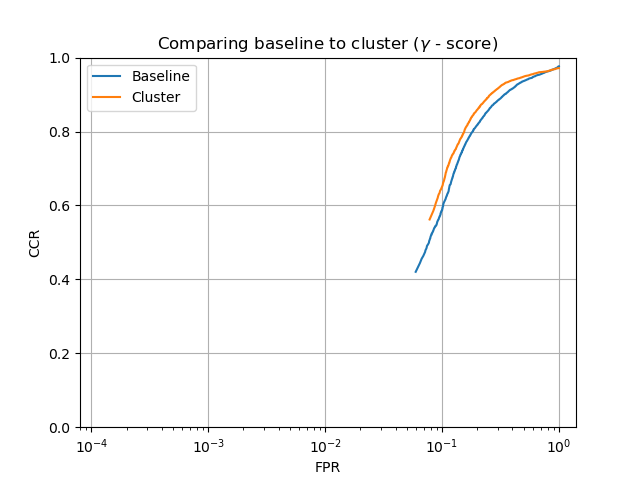
\includegraphics[width=\textwidth]{figures/compare_gamma.png}
\end{frame}

\begin{frame}{Results RQ2 ($\Sigma$)}
	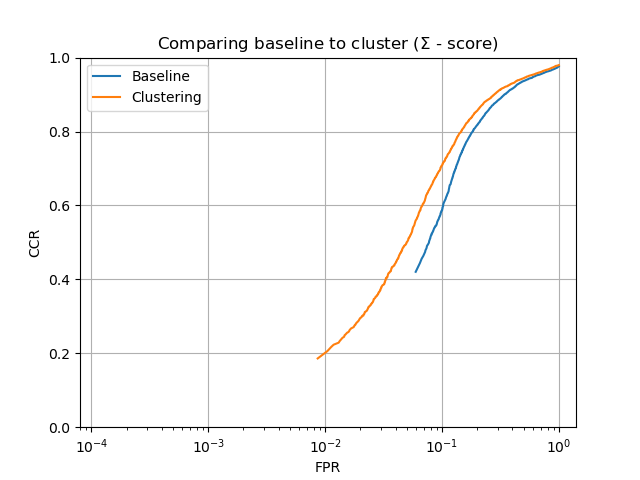
\includegraphics[width=\textwidth]{figures/compare_sigma.png}
\end{frame}

\begin{frame}{Research Questions 3}
	\texttt{RQ3}: If clustering improves OpenMax, which clustering type is optimal, and by using which parameters?
\end{frame}

\begin{frame}{Results RQ3 ($\gamma$)}
	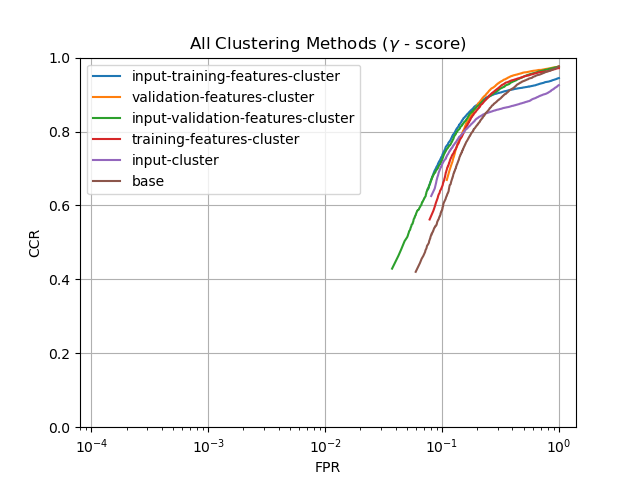
\includegraphics[width=\textwidth]{figures/all_methods_gamma.png}
\end{frame}

\begin{frame}{Results RQ3 ($\Sigma$)}
	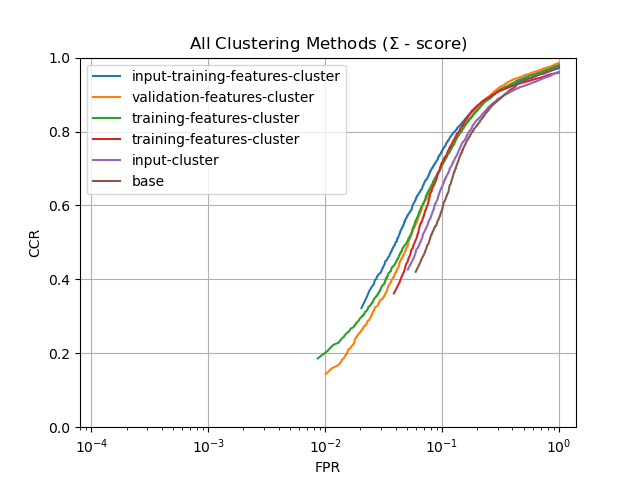
\includegraphics[width=\textwidth]{figures/all_methods_sigma.png}
\end{frame}
